\subsection{Simulating Your Designs}
We have provided functional test benches for both the top level module and the lower level CRC calculator. This works for now; however, to verify your results before submitting you will want to simulate them. Make sure that the CRC Testbench is setup as the top level simulator.

\begin{figure}[H]
    \centering
    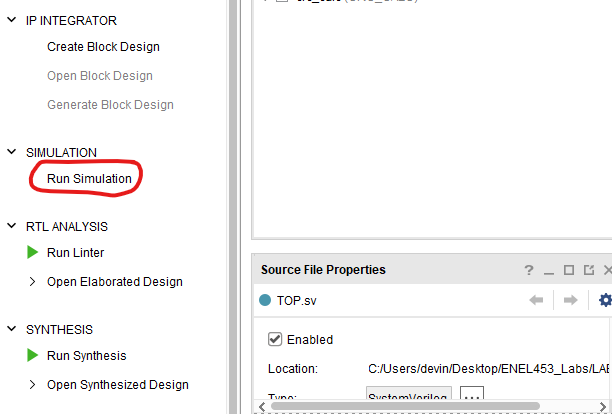
\includegraphics[width=7cm]{Images/SimulatingDesign/Run_Simulation_Page1.png}
    \caption{Press Run Simulation and select Run Behavioral Simulation}
    \label{fig:enter-label}
\end{figure}
To simulate the CRC Code calculator select Run Simulation on the side, then select run behavioral simulation. 
\begin{figure}[H]
    \centering
    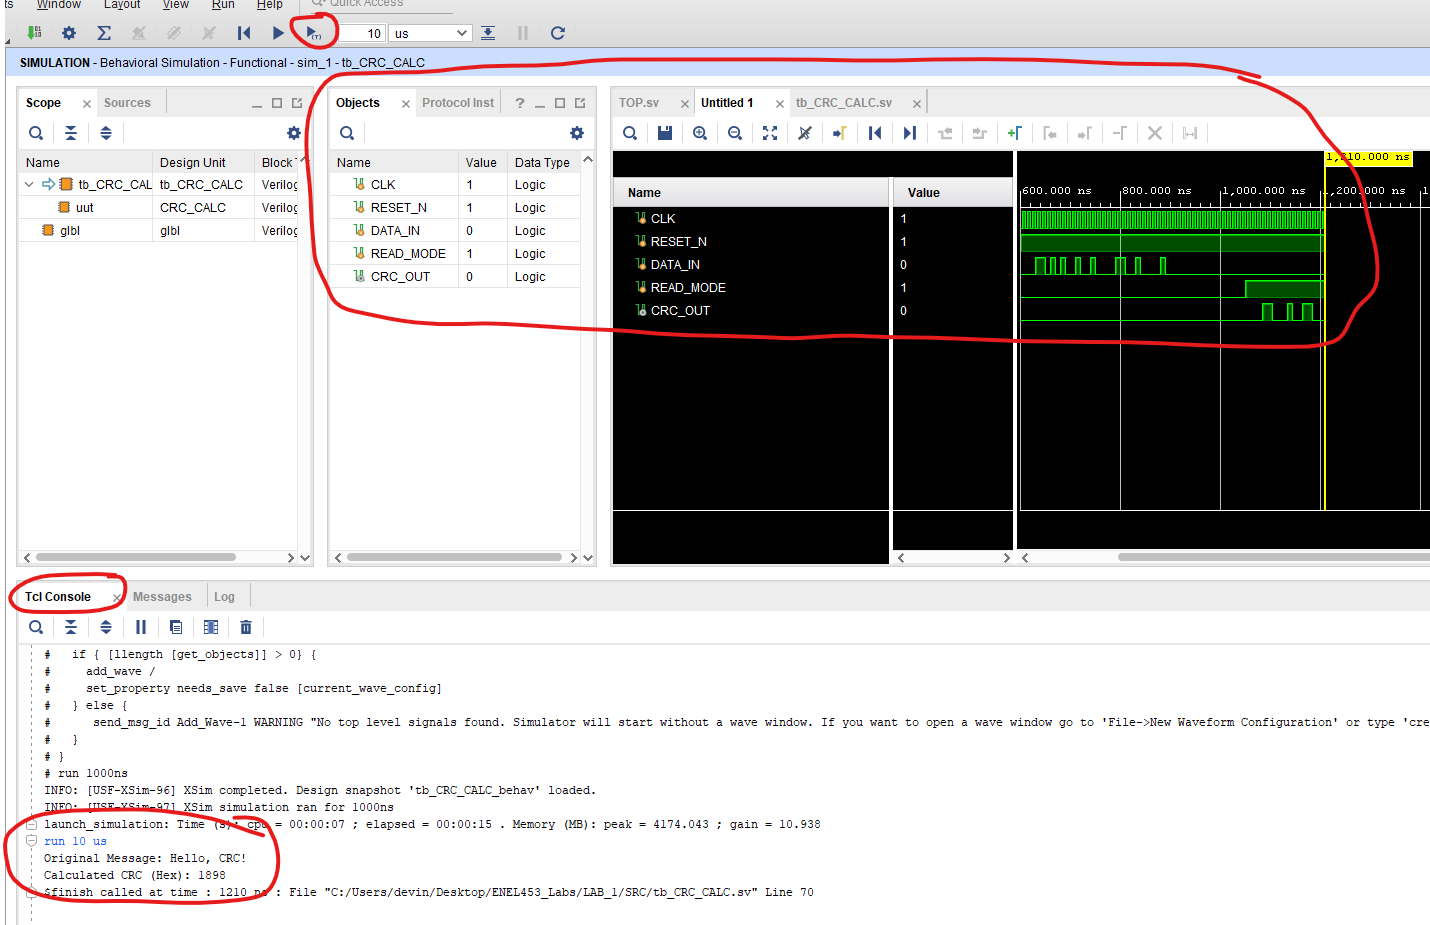
\includegraphics[width=7cm]{Images/SimulatingDesign/Run_Simulation_Page2.png}
    \caption{Your Simulation should run}
    \label{fig:enter-label}
\end{figure}
The simulation will run for a short time and then stop part way. Click the button up at the top next to the play button to run for an additional 10\begin{math}\mu\end{math}s. This will run the simulation through calculating the CRC value. In the large window you will be able to see the different signals changing over time. If you select the TCL console you will see that your simulation printed 2 lines of text.\\
\begin{verbatim}
    Original Message: Hello, CRC!
    Calculated CRC (Hex): 1898
\end{verbatim}
You can calculate the XMODEM CRC check value for the text and you'll find the value is correct for the input text. 